\begin{figure}
  \centering
  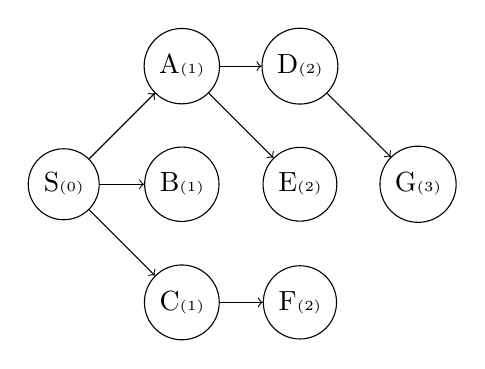
\begin{tikzpicture}[->, auto, node distance=1.5cm, every node/.style={circle, draw, minimum size=.5cm}]
    \node (S) {S\tiny{(0)}};
    \node (B) [right of=S] {B\tiny{(1)}};
    \node (A) [above of=B] {A\tiny{(1)}};
    \node (C) [below of=B] {C\tiny{(1)}};
    \node (D) [right of=A] {D\tiny{(2)}};
    \node (E) [below of=D] {E\tiny{(2)}};
    \node (F) [below of=E] {F\tiny{(2)}};
    \node (G) [right of=E] {G\tiny{(3)}};

    \path[every node]
    (S) edge (A)
    (S) edge (B)
    (S) edge (C)
    (A) edge (D)
    (A) edge (E)
    (C) edge (F)
    (D) edge (G)
    ;
  \end{tikzpicture}
\end{figure}